%--------------------------------------------------
\subsection{Prototipo 3: Integración con servidor (Detalles y estadísticas de clientes y envío de recomendaciones)}

El prototipo 3 de la aplicación incluye las modificaciones en el diseño inicial de la aplicación para mostrar los detalles y estadísticas de un cliente cercano al vendedor y la integración de la aplicación con los servicios REST para obtener dichos datos. De igual forma dentro de este prototipo se incluye el diseño para que el vendedor envié recomendaciones de productos del departamento actual a un cliente y su respectiva integración con el servidor para el envió de las mismas en forma de notificación por medio de Firebase Cloud Messaging (FCM). \\ \par

%--------------------------------------------------

\subsubsection{Análisis}

Dentro del análisis para el desarrollo de este prototipo se incorporan los requerimientos funcionales \hyperlink{RFAPV}{RFAPV5 Obtener detalles y estadísticas de un cliente} y \hyperlink{RFAPV}{RFAPV6 Enviar recomendaciones a clientes}, definidos previamente en el capítulo del ``Bosquejo general de la aplicación''  con el título de ``Requerimientos funcionales de la Aplicación Interactiva para el Personal de Ventas''. \\ \par

\paragraph{Casos de uso de la AIPV.} ~\\

La figura \ref{casos-uso-AIPV1} definida previamente en el prototipo 1, muestra los casos de uso de la AIPV.

\paragraph{Diagrama de clases.} ~\\

La figura \ref{clases-AIPV3} presenta el diagrama de clases para el prototipo 3 de la AIPV. Para una mejor visualización, el diagrama se ha dividido en 3 partes. 

\FloatBarrier
\begin{figure}[htbp!]
		\centering
			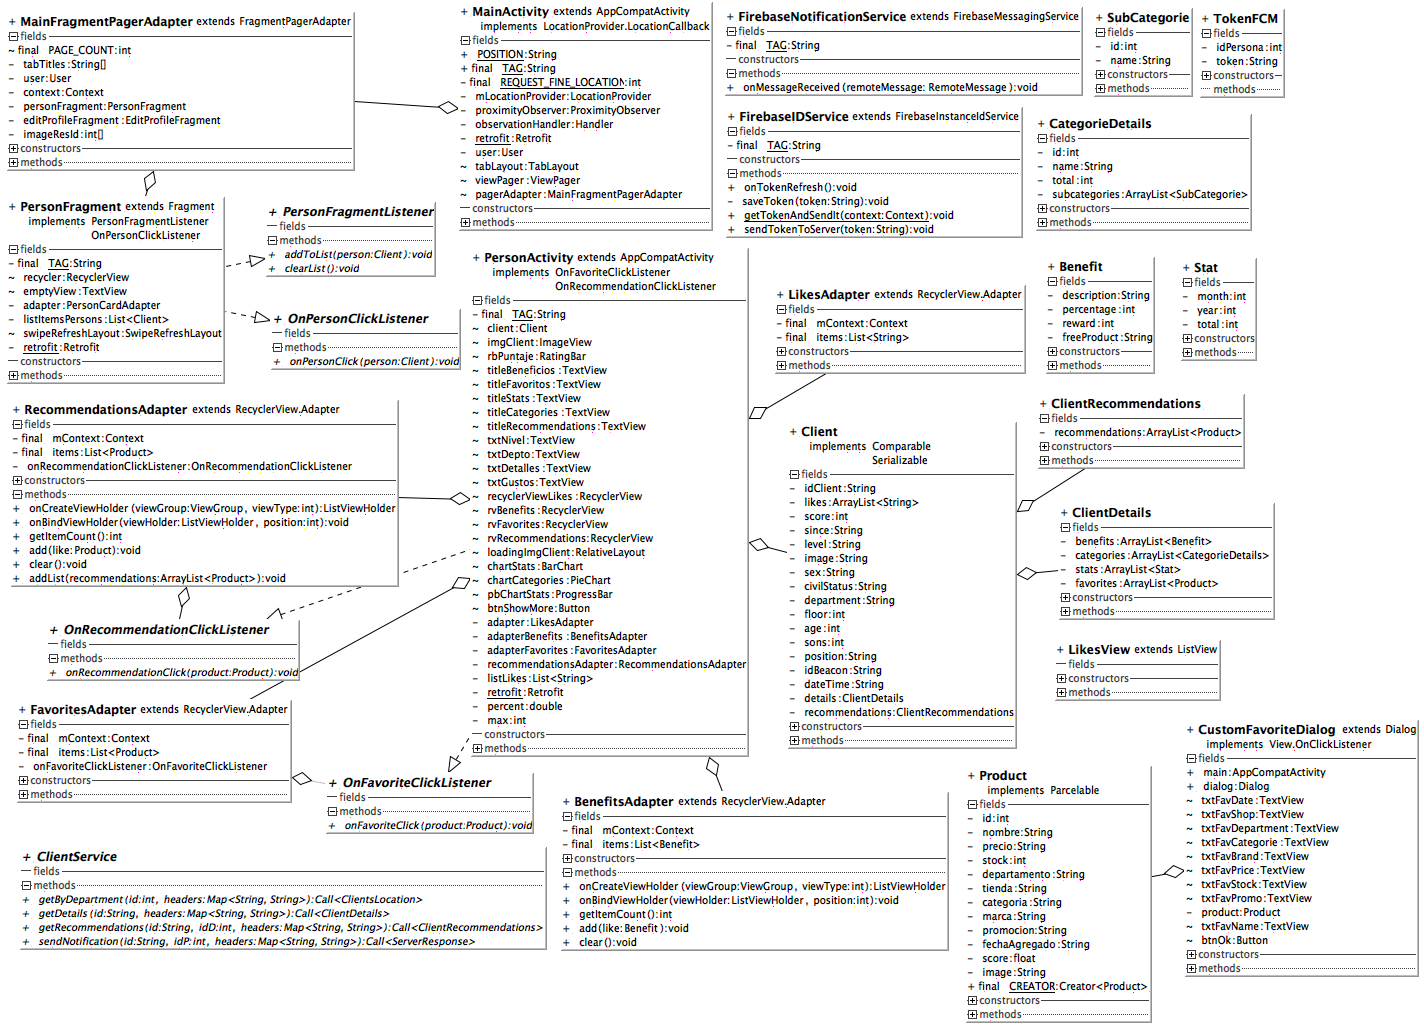
\includegraphics[width=1 \textwidth]{imagenes/adrian/vendedor/prototipo3/clases}
		\caption{Diagrama de clases del prototipo 3 de la AIPV (Visualización completa).}
		\label{clases-AIPV3}
\end{figure}
\FloatBarrier

La descripción de los nuevos elementos de la figura \ref{clases-AIPV3-parte1} es la siguiente: 

\begin{itemize}
\item \textbf{PersonActivity}: Versión actualizada de la clase que extiende de AppCompatActivity y en la que se muestran los detalles de un cliente.
\item \textbf{RecommendationsAdapter}: Clase que extiende de RecyclerView.Adapter y funciona como el adaptador del arreglo de recomendaciones de productos del departamento actual que le podrían interesar al cliente del cual se están mostrando sus detalles. 
\item \textbf{OnRecommendationClickListener}: Interfaz que define el método onRecommendationClick el cual recibe un producto seleccionado por el vendedor para ser enviado como recomendación al cliente.
\end{itemize}

\FloatBarrier
\begin{figure}[htbp!]
		\centering
			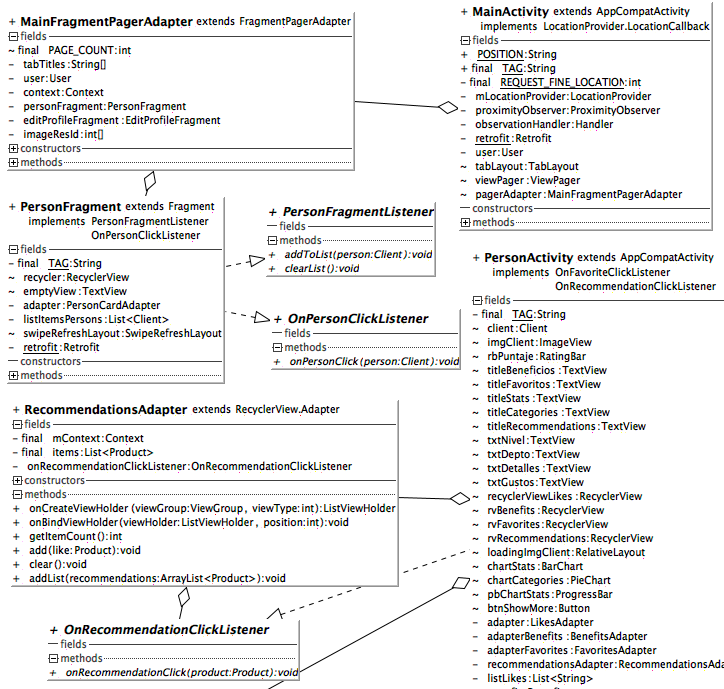
\includegraphics[width=.8 \textwidth]{imagenes/adrian/vendedor/prototipo3/clases_1}
		\caption{Diagrama de clases del prototipo 3 de la AIPV (Parte 1) .}
		\label{clases-AIPV3-parte1}
\end{figure}
\FloatBarrier

La descripción de los nuevos elementos de la figura \ref{clases-AIPV3-parte2} es la siguiente: 

\begin{itemize}
\item \textbf{FirebaseNotificationService}: Clase que extiende de FirebaseMessagingService y que nos permite recibir cualquier notificación en la aplicación.
\item \textbf{FirebaseIDService}: Clase que extiende de FirebaseInstanceIdService y funciona para obtener el token actual de Firebase Cloud Messaging para el dispositivo.
\item \textbf{TokenFCM}: Clase POJO que se utiliza para relacionar al vendedor con la sesión actual y el token de Firebase Cloud Messaging que se genera en la aplicación lo cual se envía en formato JSON al servidor para actualizar dicho token.
\item \textbf{ClientDetails}: Clase POJO que contiene todos los detalles de un cliente: beneficios, categorías más compradas, estadísticas y productos favoritos.
\item \textbf{CategorieDetails}: Clase POJO que se recibe como JSON al obtener las estadísticas del cliente, en este caso sobre las categorías que más compra. 
\item \textbf{SubCategorie}: Clase POJO que representa una subcategoría, estás subcategorías se encuentran en forma de arreglo dentro de cada una de las categorías que más compra un cliente.
\item \textbf{Benefit}: Clase POJO que contiene los datos necesarios de un beneficio de acuerdo al nivel del cliente, se encuentra en forma de arreglo dentro de los detalles del cliente.
\item \textbf{Stat}: Clase POJO, especifica el total de compras que realizó el cliente en un año y mes específicos, se encuentra en forma de arreglo dentro de los detalles del cliente. 
\item \textbf{ClientRecommendations}: Clase POJO que se recibe como JSON después de obtener las estadísticas del cliente, contiene un arreglo de productos del departamento que podrían gustarle al cliente.
\item \textbf{LikesAdapter}: Clase que extiende de RecyclerView.Adapter y funciona como el adaptador del arreglo de los gustos de un cliente que se muestran en forma de lista horizontal.
\item \textbf{LikesView}: Clase que extiende de ListView y nos permite configurar el tamaño de la vista que se ocupa para desplegar los gustos del cliente en forma de lista.
\end{itemize}

\FloatBarrier
\begin{figure}[htbp!]
		\centering
			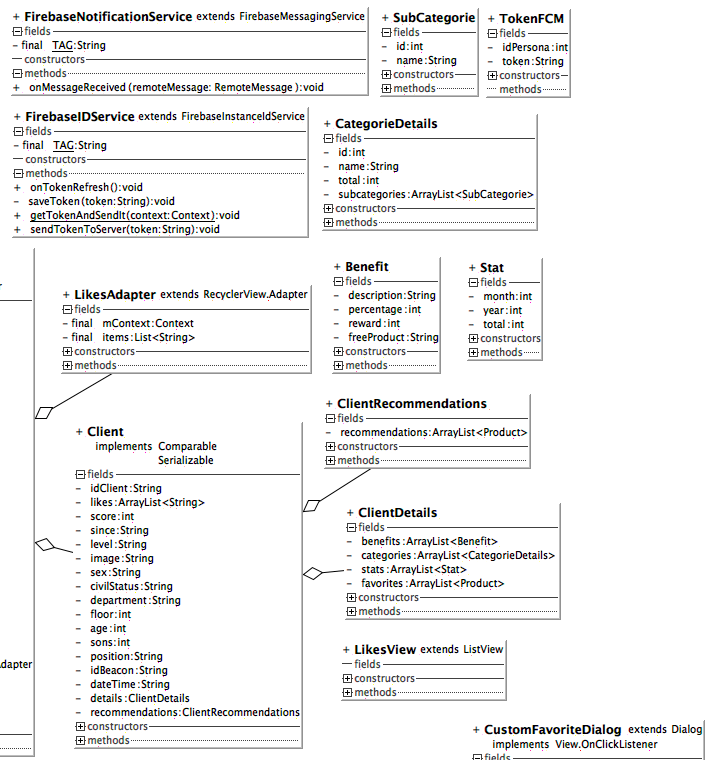
\includegraphics[width=.8 \textwidth]{imagenes/adrian/vendedor/prototipo3/clases_2}
		\caption{Diagrama de clases del prototipo 3 de la AIPV (Parte 2) .}
		\label{clases-AIPV3-parte2}
\end{figure}
\FloatBarrier

La descripción de los nuevos elementos de la figura \ref{clases-AIPV3-parte3} es la siguiente: 

\begin{itemize}
\item \textbf{FavoritesAdapter}: Clase que extiende de RecyclerView.Adapter y funciona como el adaptador del arreglo de productos favoritos de un cliente que se muestran en forma de lista horizontal.
\item \textbf{OnFavoriteClickListener}: Interfaz que define el método onFavoriteClick, la interfaz se implementa en la clase PersonActivity y sirve para mostrar el dialogo CustomFavoriteDialog en el cual se muestra la descripción del producto.
\item \textbf{BenefitsAdapter}:  Clase que extiende de RecyclerView.Adapter y funciona como el adaptador del arreglo de beneficios de un cliente que se muestran en forma de lista horizontal.
\item \textbf{Product}: La clase POJO actualizada que incorpora ahora los nuevos atributos score y image, los cuales se muestran en los productos que se podrían recomendar al cliente.
\item \textbf{CustomFavoriteDialog}: Clase que extiende de Dialog y la cual se utiliza para mostrar los detalles de un producto que el cliente tiene en favoritos. 
\end{itemize}

\FloatBarrier
\begin{figure}[htbp!]
		\centering
			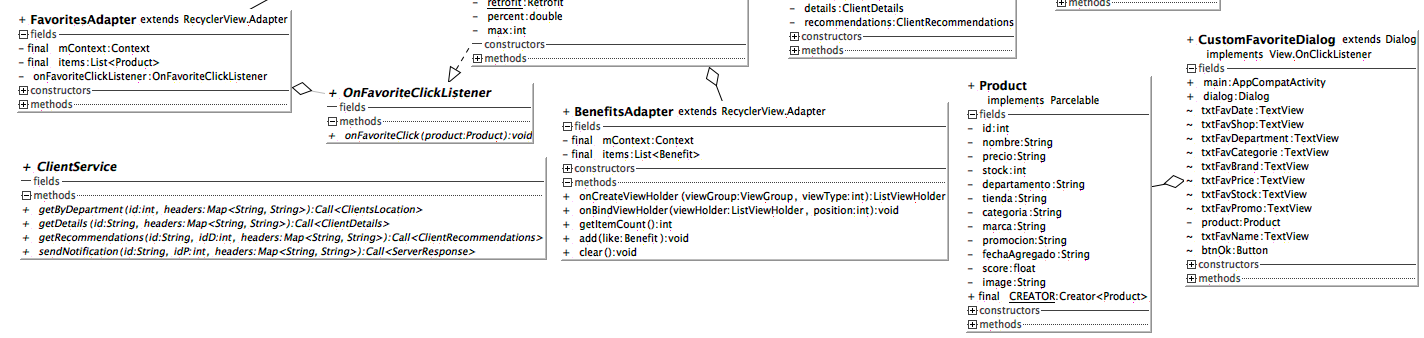
\includegraphics[width=1 \textwidth]{imagenes/adrian/vendedor/prototipo3/clases_3}
		\caption{Diagrama de clases del prototipo 3 de la AIPV (Parte 3) .}
		\label{clases-AIPV3-parte3}
\end{figure}
\FloatBarrier

%--------------------------------------------------
\subsubsection{Diseño}

A partir de los requerimientos definidos para este prototipo se muestran los diagramas de secuencia.\\ \par

\paragraph{Diagramas de secuencia.} ~\\

\title{\textbf{Obtener estadísticas del cliente.}\\}

En la figura \ref{secuencia-AIPV3-detalles} se muestra el diagrama de secuencia para obtener las estadísticas de un cliente, el cual describe los pasos que se llevan a cabo para que el usuario vendedor pueda ver información adicional del cliente como beneficios por su nivel, 5 de sus productos favoritos, el total de compras realizadas en los últimos 6 meses y las categorías de productos más compradas. Estos datos se muestran únicamente si el cliente otorga los permisos para cada uno de ellos. Para una mejor visualización el diagrama se ha dividido en 2 partes las cuales se muestran en las figuras \ref{secuencia-AIPV3-detallesUno} y \ref{secuencia-AIPV3-detallesDos} .

\FloatBarrier
\begin{figure}[htbp!]
		\centering
			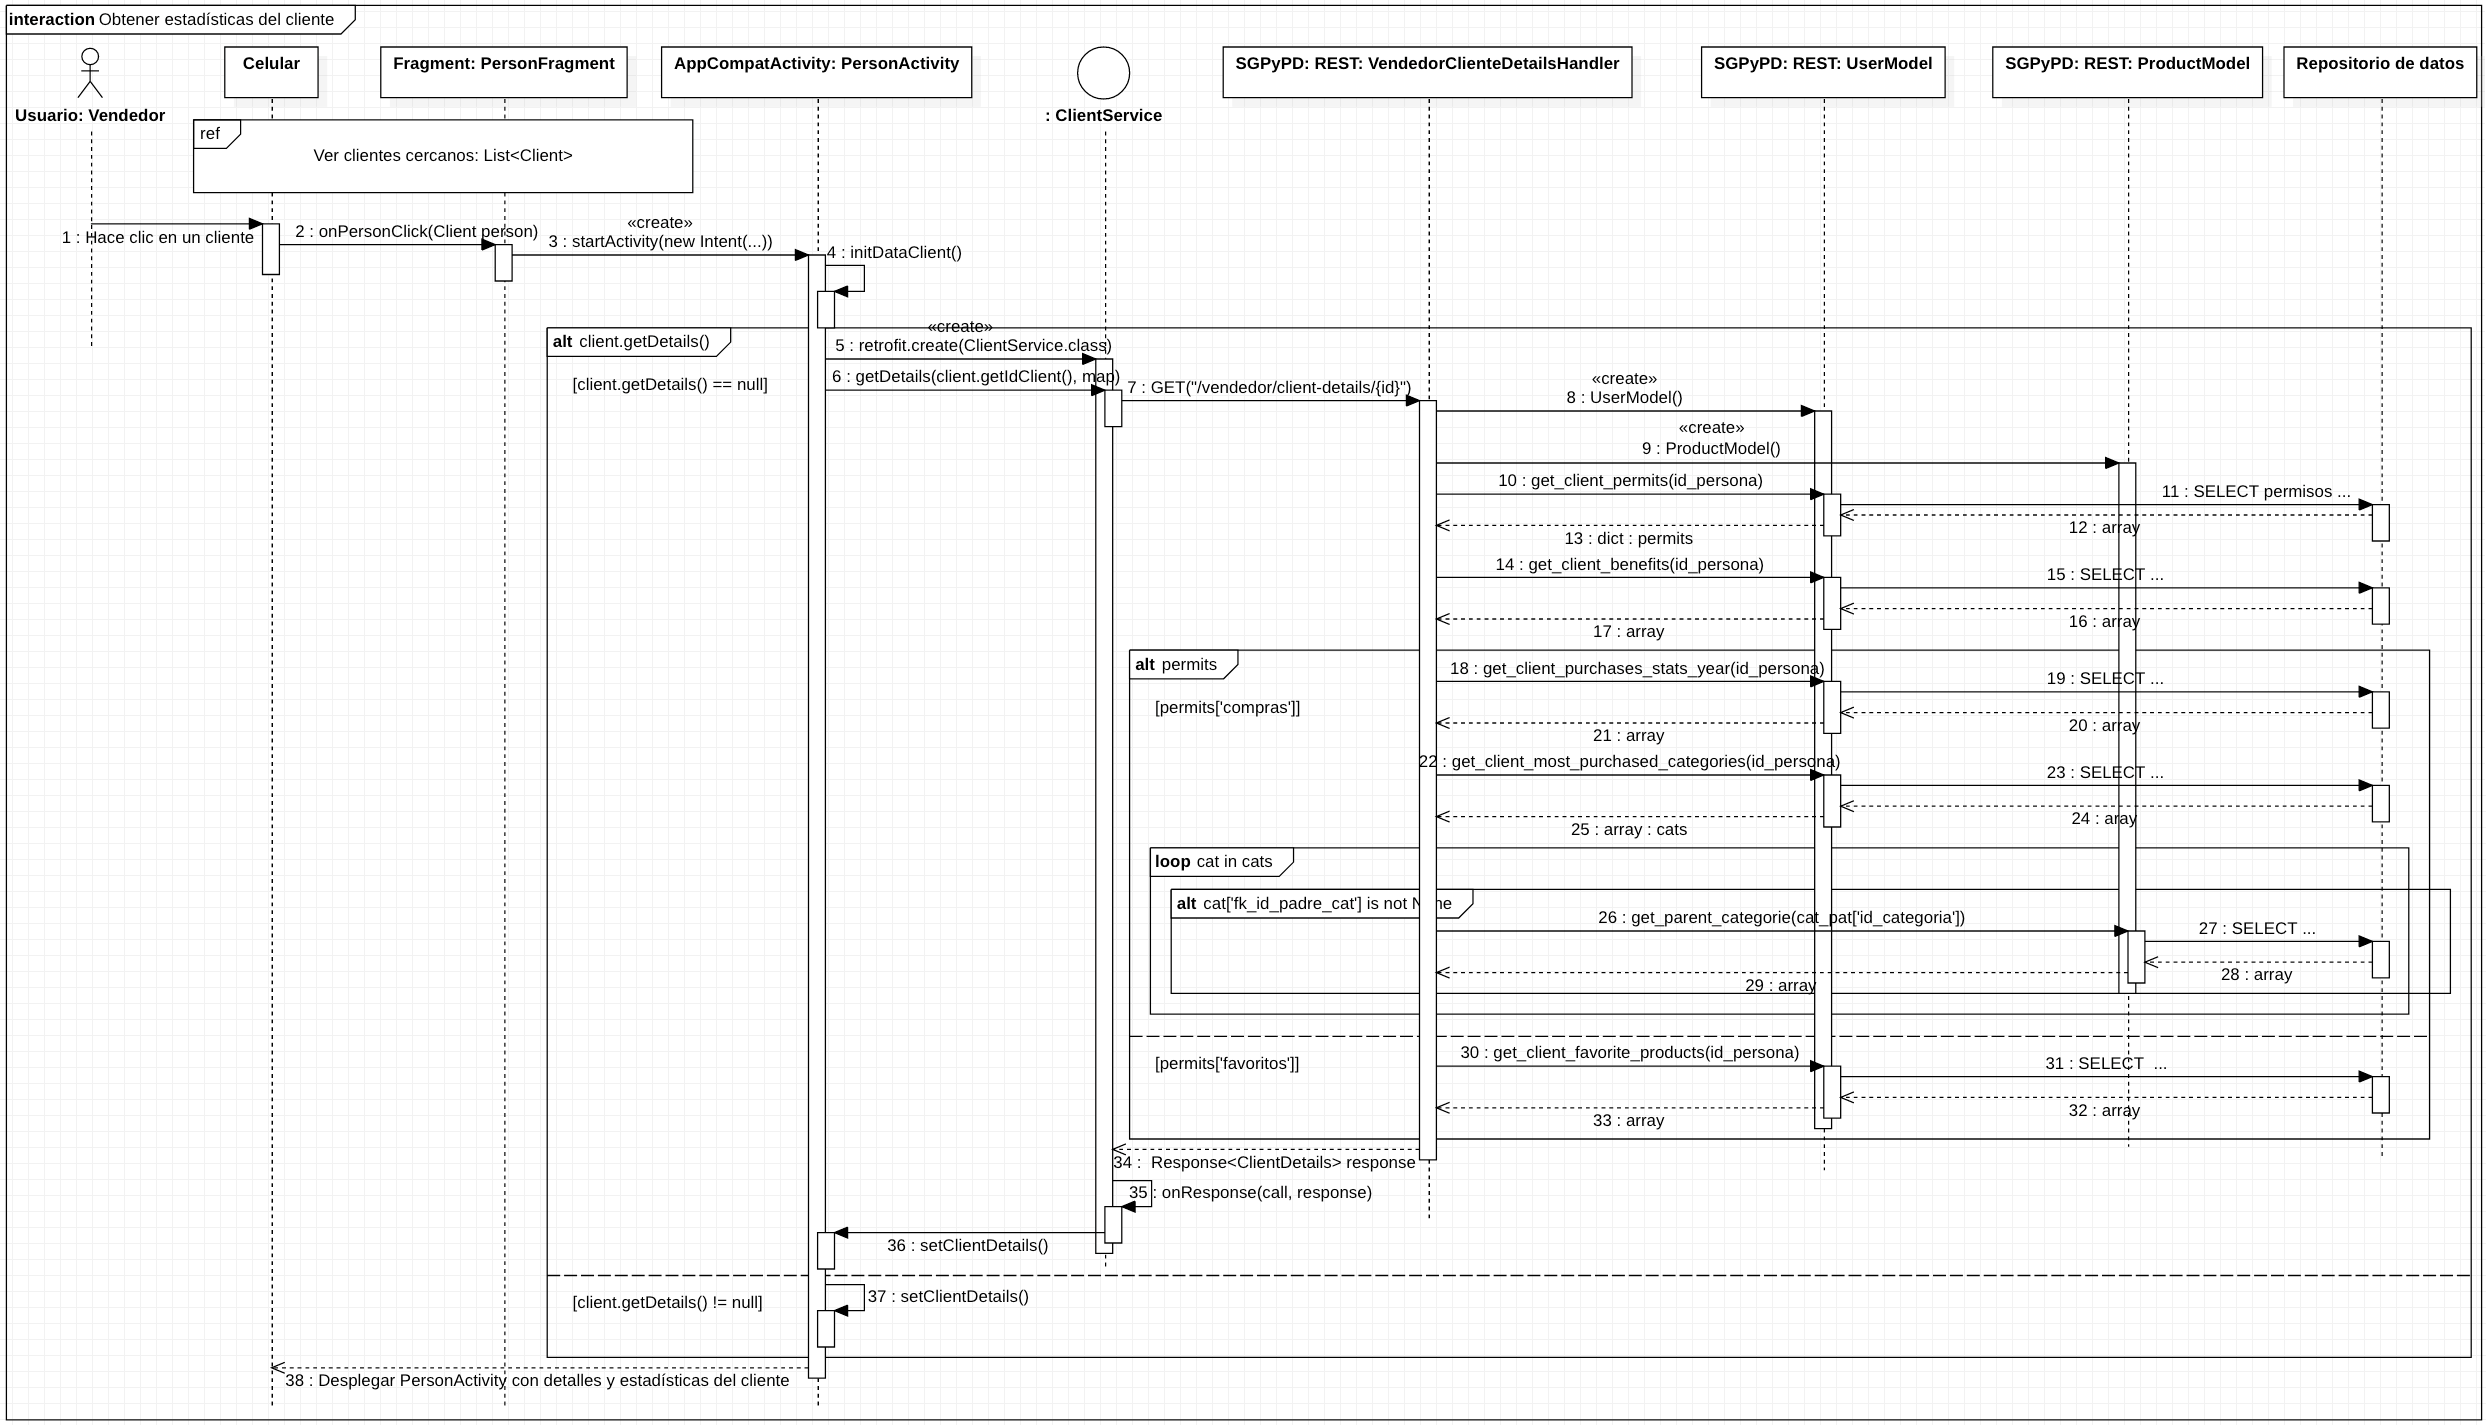
\includegraphics[width=1 \textwidth]{imagenes/adrian/vendedor/prototipo3/detallesCliente}
		\caption{Diagrama de secuencia para obtener estadísticas de un cliente.}
		\label{secuencia-AIPV3-detalles}
\end{figure}
\FloatBarrier

\FloatBarrier
\begin{figure}[htbp!]
		\centering
			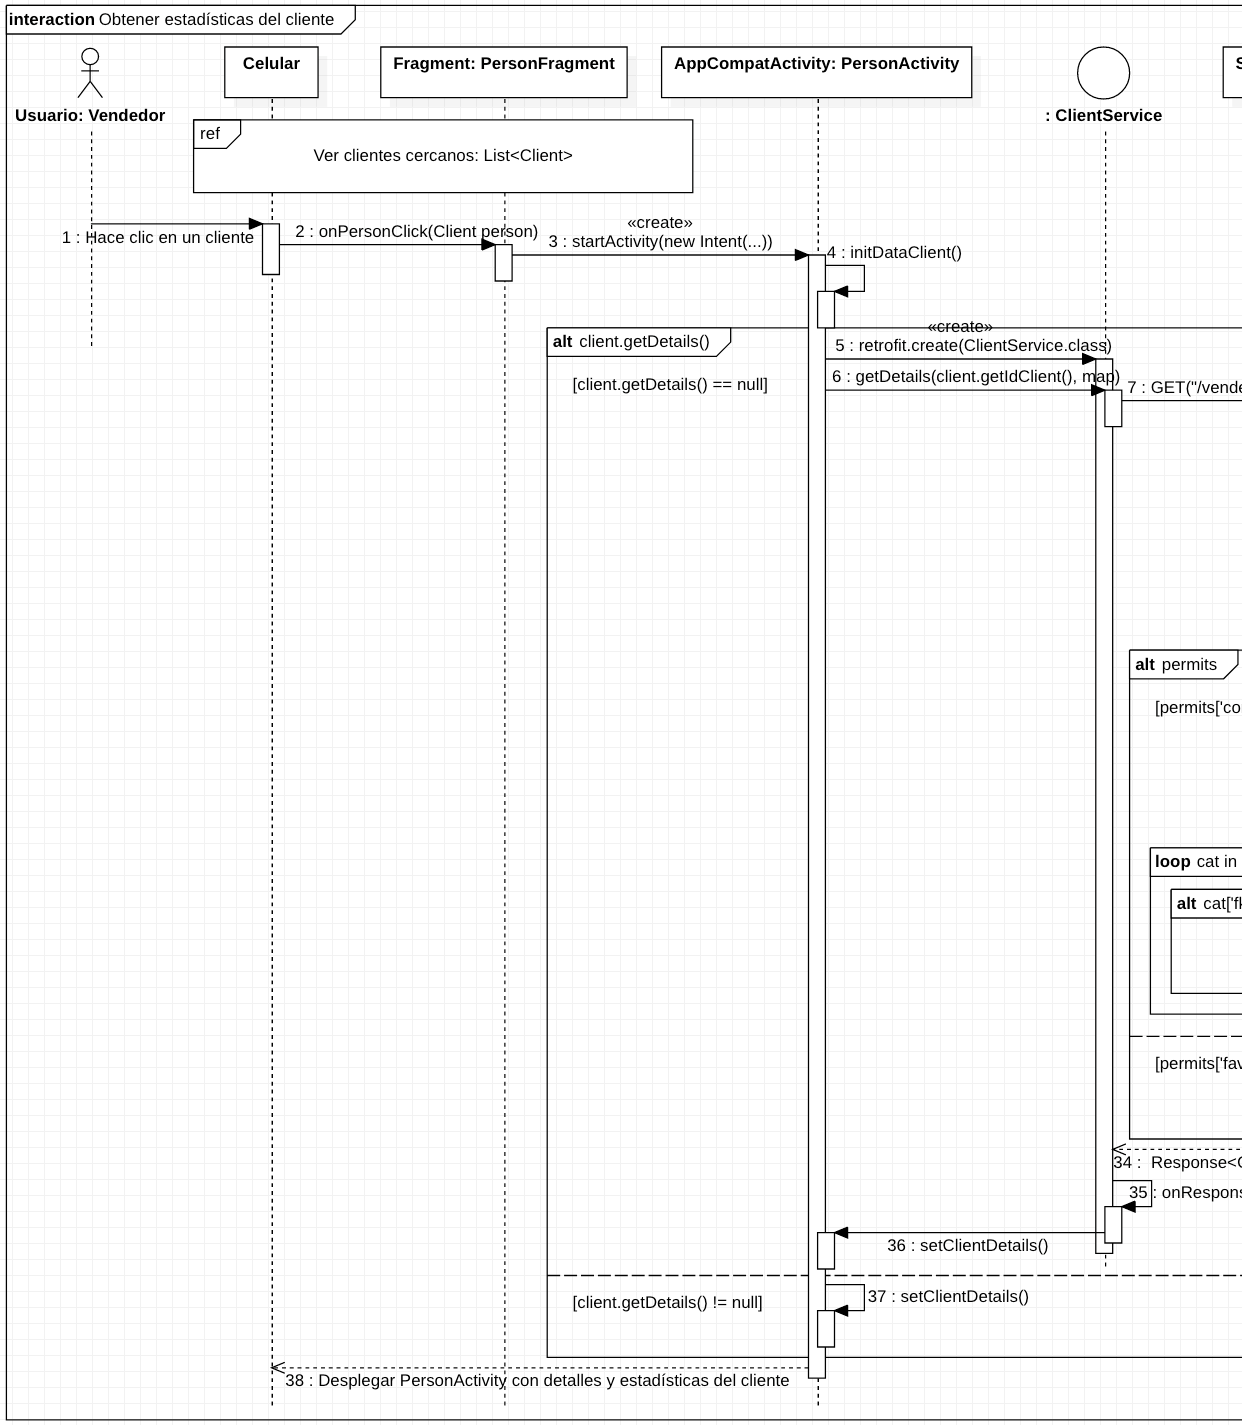
\includegraphics[width=1 \textwidth]{imagenes/adrian/vendedor/prototipo3/detallesCliente1}
		\caption{Diagrama de secuencia para obtener estadísticas de un cliente (Parte 1).}
		\label{secuencia-AIPV3-detallesUno}
\end{figure}
\FloatBarrier

\FloatBarrier
\begin{figure}[htbp!]
		\centering
			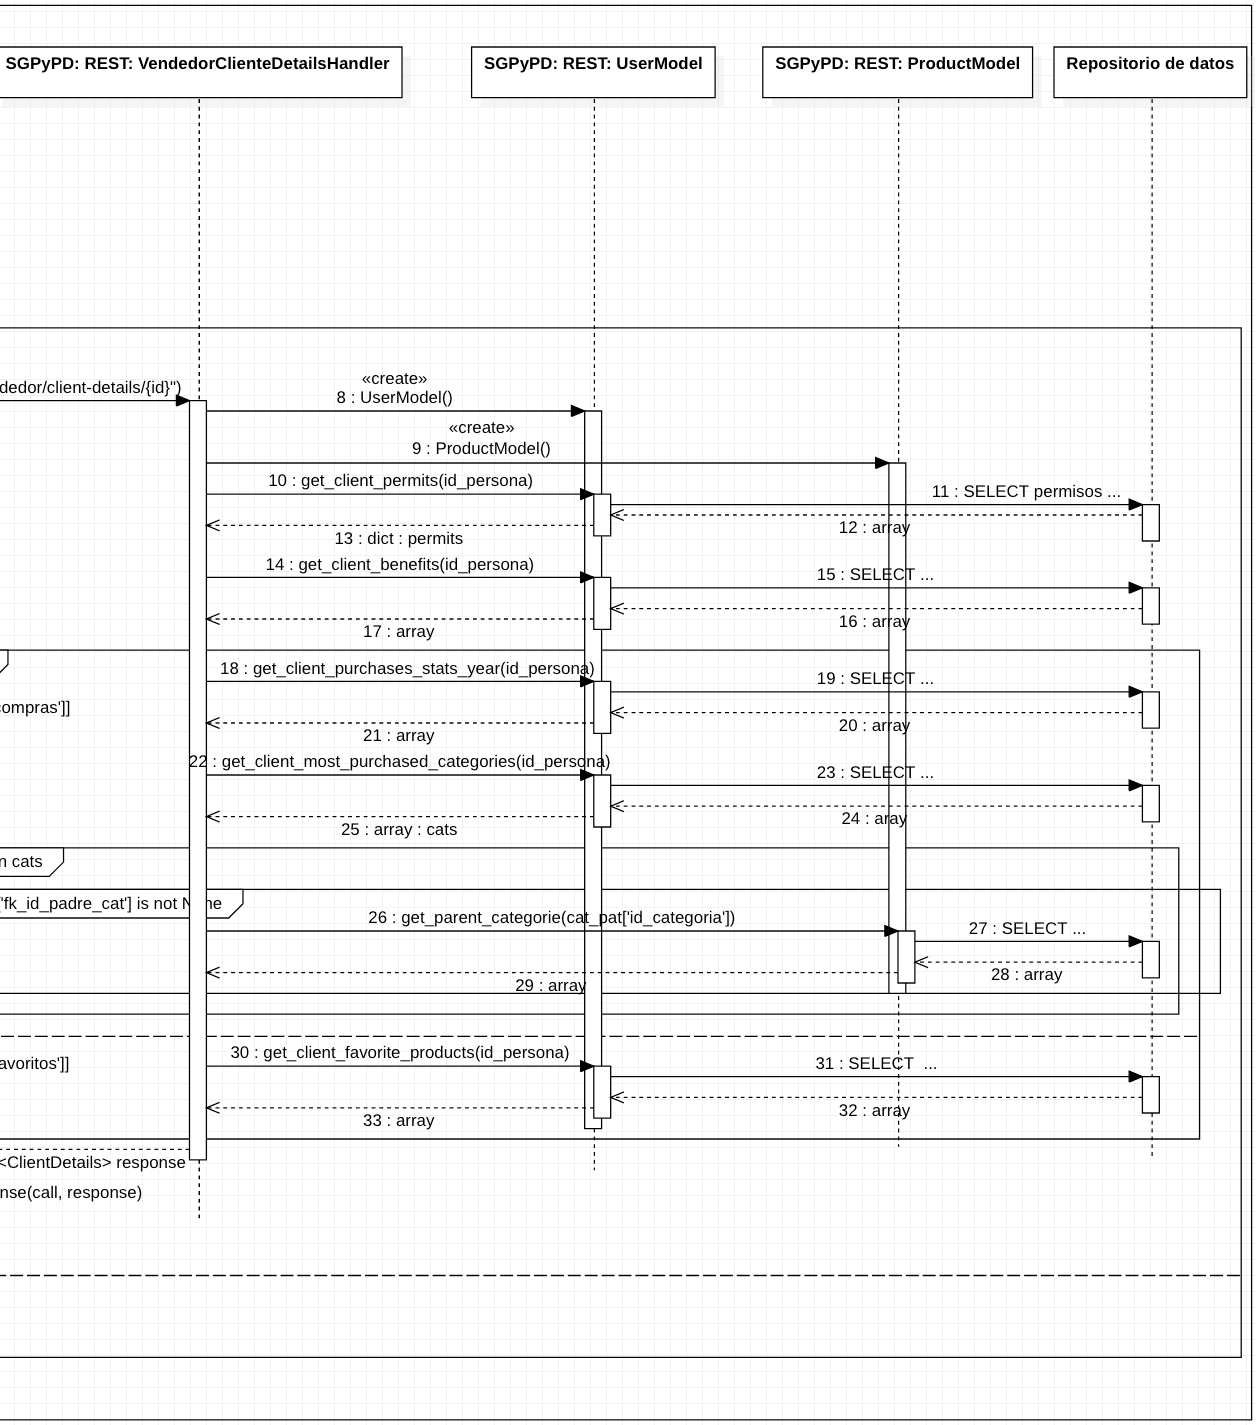
\includegraphics[width=1 \textwidth]{imagenes/adrian/vendedor/prototipo3/detallesCliente2}
		\caption{Diagrama de secuencia para obtener estadísticas de un cliente (Parte 2).}
		\label{secuencia-AIPV3-detallesDos}
\end{figure}
\FloatBarrier

\title{\textbf{Obtener recomendaciones para cliente.}\\}

En la figura \ref{secuencia-AIPV3-obtenRecom} se muestra el diagrama de secuencia para obtener recomendaciones de productos para un cliente exclusivamente para el departamento en el que se encuentra, esto ocurre acto seguido de que se obtienen las estadísticas del cliente del servidor por lo que se coloca al inicio como referencia el diagrama de secuencia ``Obtener estadísticas del cliente''. Para una mejor visualización el diagrama se ha dividido en 2 partes las cuales se muestran en las figuras \ref{secuencia-AIPV3-obtenRecomUno} y \ref{secuencia-AIPV3-obtenRecomDos} .

\FloatBarrier
\begin{figure}[htbp!]
		\centering
			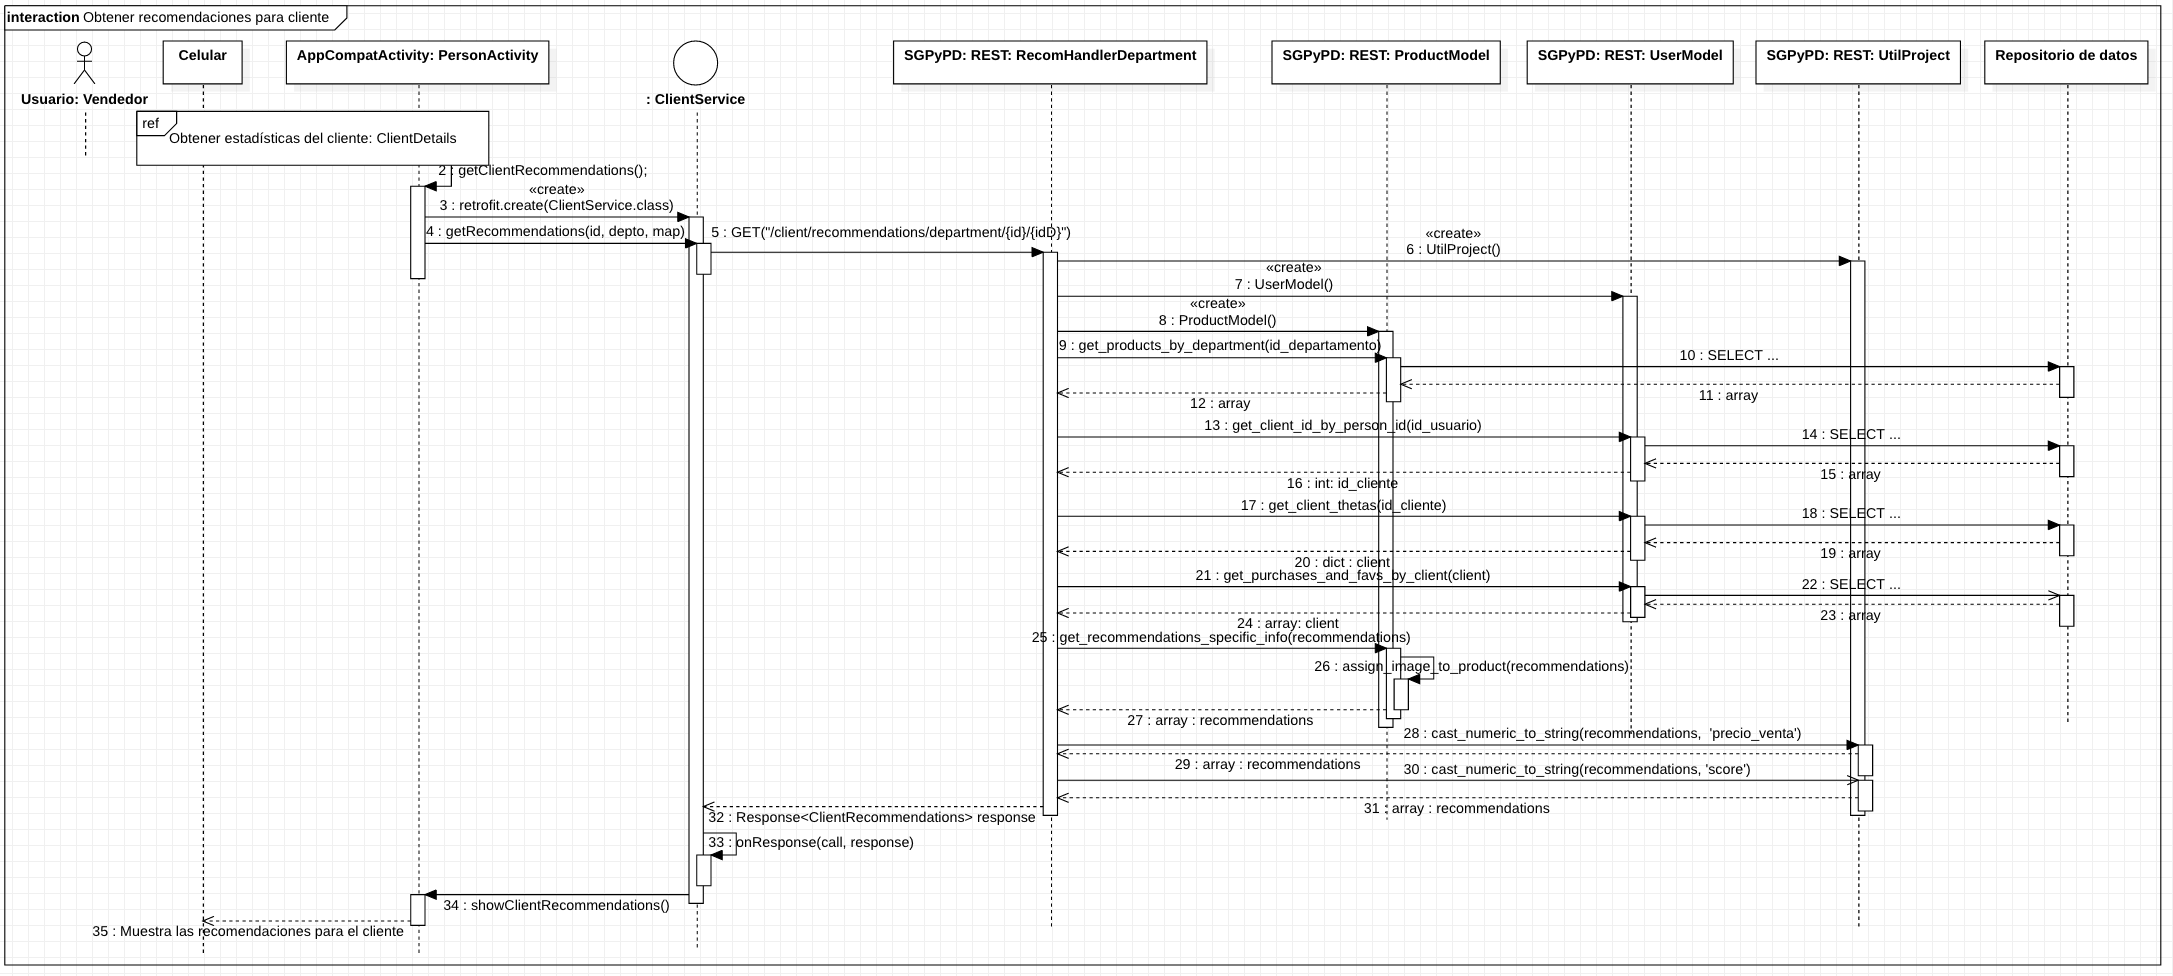
\includegraphics[width=1 \textwidth]{imagenes/adrian/vendedor/prototipo3/obtenerRecomendaciones}
		\caption{Diagrama de secuencia para obtener recomendaciones para un cliente.}
		\label{secuencia-AIPV3-obtenRecom}
\end{figure}
\FloatBarrier

\FloatBarrier
\begin{figure}[htbp!]
		\centering
			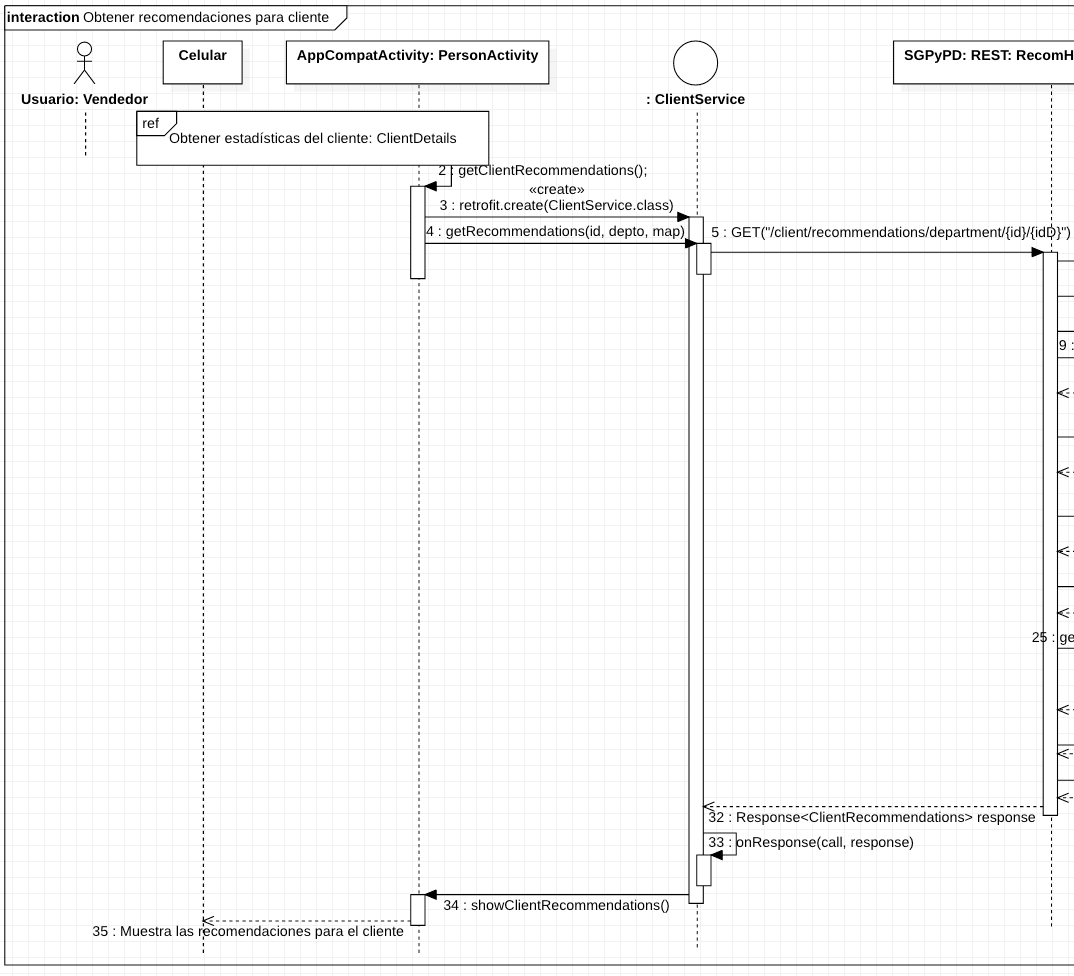
\includegraphics[width=1 \textwidth]{imagenes/adrian/vendedor/prototipo3/obtenerRecomendaciones1}
		\caption{Diagrama de secuencia para obtener recomendaciones para un cliente (Parte 1).}
		\label{secuencia-AIPV3-obtenRecomUno}
\end{figure}
\FloatBarrier

\FloatBarrier
\begin{figure}[htbp!]
		\centering
			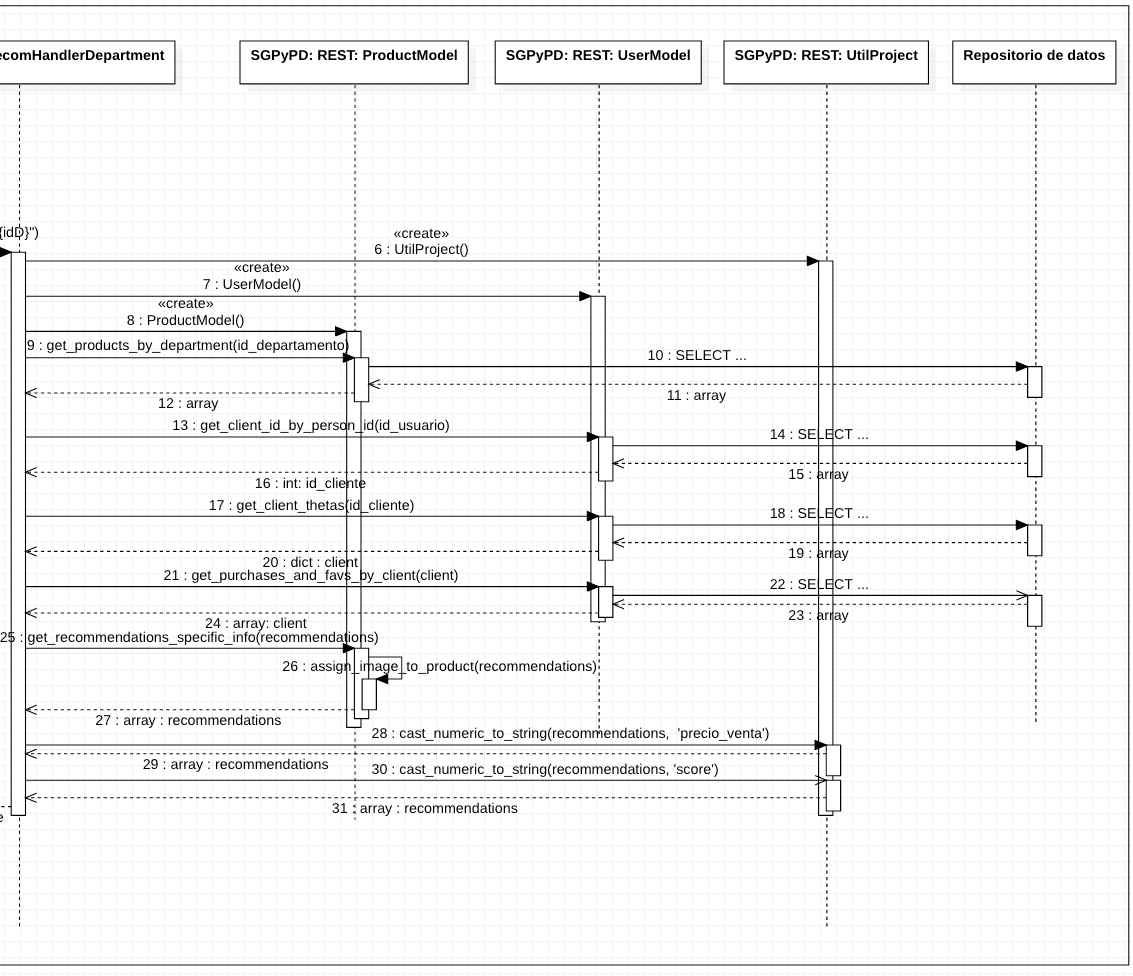
\includegraphics[width=1 \textwidth]{imagenes/adrian/vendedor/prototipo3/obtenerRecomendaciones2}
		\caption{Diagrama de secuencia para obtener recomendaciones para un cliente (Parte 2).}
		\label{secuencia-AIPV3-obtenRecomDos}
\end{figure}
\FloatBarrier

\title{\textbf{Enviar recomendaciones al cliente.}\\}

En la figura \ref{secuencia-AIPV3-recom} se muestra el diagrama de secuencia para enviar recomendaciones a un cliente, el cual describe los pasos que se llevan a cabo para que el usuario vendedor pueda enviar una recomendación de un producto del departamento actual al cliente mediante una notificación de Firebase Cloud Messaging (FCM), es importante mencionar que esto ocurre después de que se obtienen las recomendaciones para el cliente por lo que se coloca al inicio como referencia el diagrama de secuencia ``Obtener recomendaciones para cliente''. Para una mejor visualización el diagrama se ha dividido en 2 partes las cuales se muestran en las figuras \ref{secuencia-AIPV3-recomUno} y \ref{secuencia-AIPV3-recomDos} .

\FloatBarrier
\begin{figure}[htbp!]
		\centering
			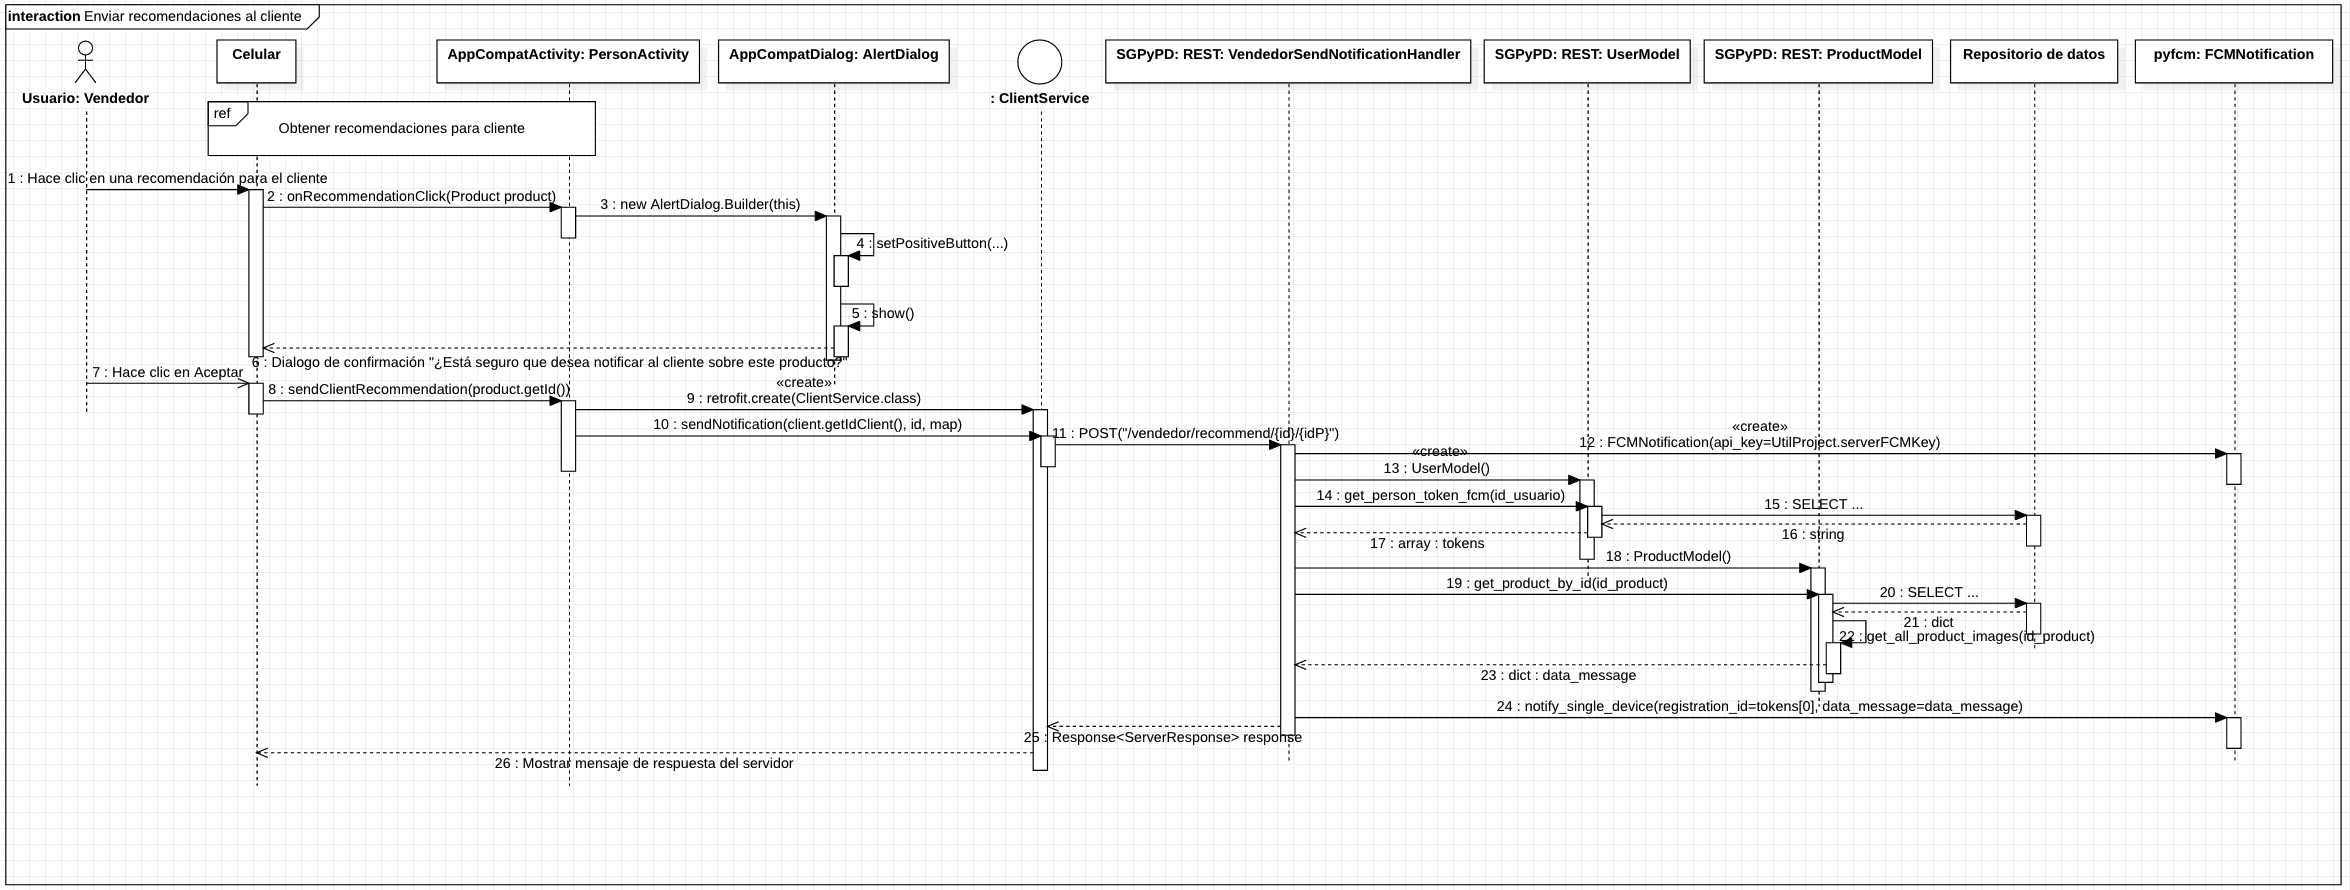
\includegraphics[width=1 \textwidth]{imagenes/adrian/vendedor/prototipo3/enviarRecomendaciones}
		\caption{Diagrama de secuencia para enviar recomendaciones a un cliente.}
		\label{secuencia-AIPV3-recom}
\end{figure}
\FloatBarrier

\FloatBarrier
\begin{figure}[htbp!]
		\centering
			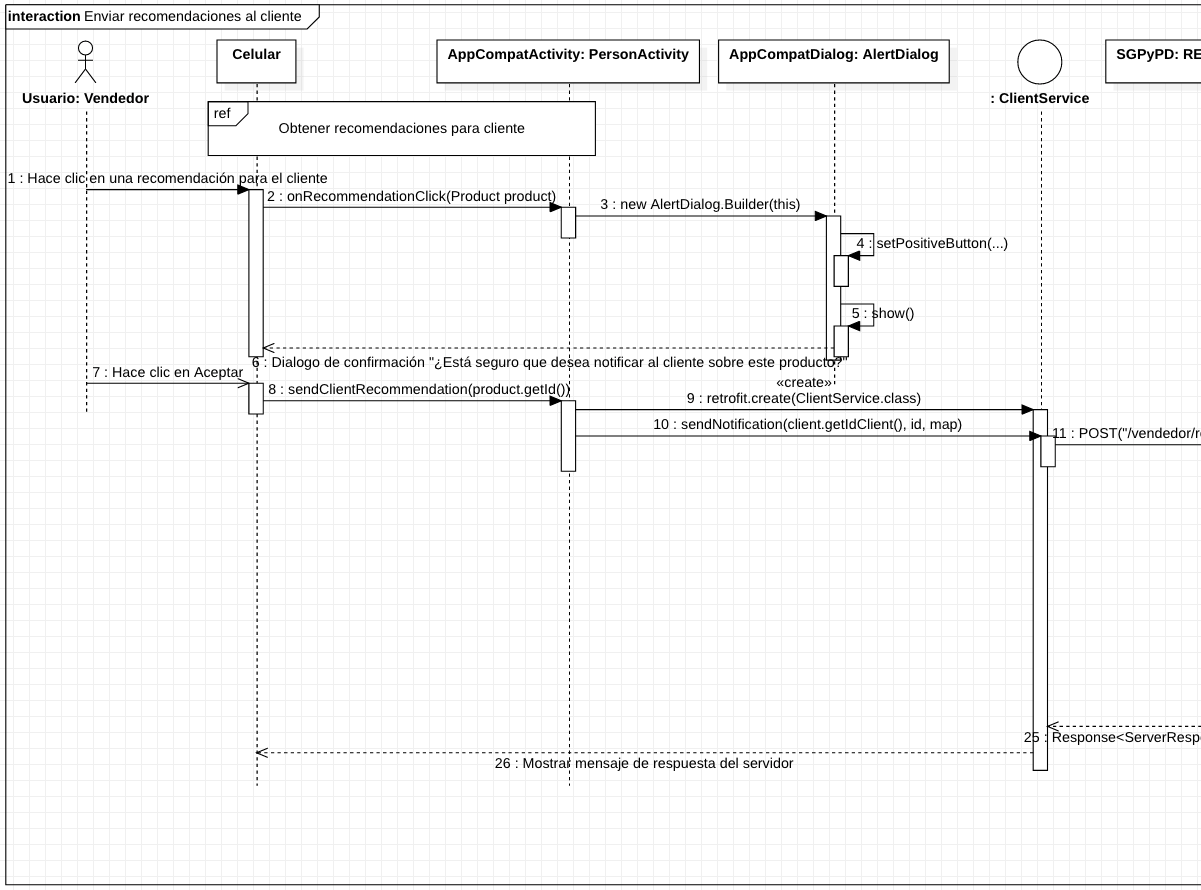
\includegraphics[width=1 \textwidth]{imagenes/adrian/vendedor/prototipo3/enviarRecomendaciones1}
		\caption{Diagrama de secuencia para enviar recomendaciones a un cliente (Parte 1).}
		\label{secuencia-AIPV3-recomUno}
\end{figure}
\FloatBarrier

\FloatBarrier
\begin{figure}[htbp!]
		\centering
			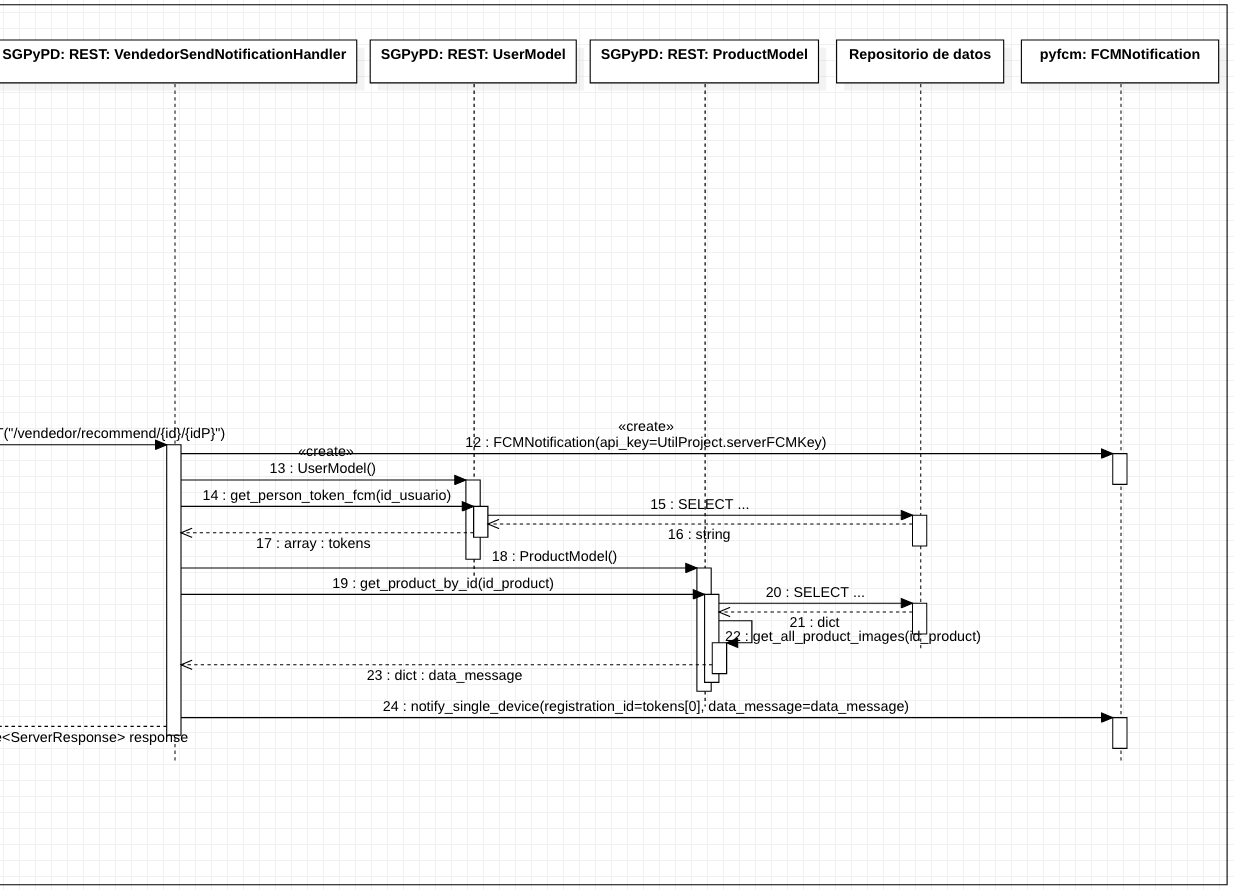
\includegraphics[width=1 \textwidth]{imagenes/adrian/vendedor/prototipo3/enviarRecomendaciones2}
		\caption{Diagrama de secuencia para enviar recomendaciones a un cliente (Parte 2).}
		\label{secuencia-AIPV3-recomDos}
\end{figure}
\FloatBarrier

%--------------------------------------------------
%\subsubsection{Pruebas}